%!TEX TS-program = pdflatex
%!TEX encoding = UTF-8 Unicode
%!TeX spellcheck = it_IT
%!TEX root = ../tesi.tex
%
\chapter{\textit{Obstacle Shadowing Model}}
\section{Il modello matematico}
Gli autori di~\cite{Carpenter:2015:OMI:2756509.2756512} riprendono il modello introdotto da Christoph Sommer et al.\ in~\cite{5720204},
nel quale la perdita di segnale dovuta a ostacoli $L_{s,o}$ dipende dall'attenuazione causata dai bordi dell'ostacolo (\textit{per-wall attenuation})
e quella derivante dalla superficie interna (\textit{per-meter attenuation}):
\begin{gather}\label{eq:osbtacle-model}
	L_{s,o} = \alpha n + \beta d_o
\end{gather}
Nella formula precedente, $n$ indica il numero di volte che il bordo dell'ostacolo viene intersecato dalla visuale (of LoS, da \textit{Line of sight}),
mentre $d_o$ è la distanza, in metri, attraversa all'interno dell'ostacolo.
Il parametro $\alpha$ rappresenta l'attenuazione per-metro espressa in decibels (dBm), invece
$\beta$ l'attenuazione per-metro, sempre in decibels  (dB/m).

I due fattori di calibrazione permettono di rappresentare più tipologie di edificio.
I valori predefiniti di $\alpha = 9$ dBm e $\beta = 0,4$ dB/m sono buoni per la maggior parte delle applicazioni
anche se, naturalmente, non per tutte.
Riportando l'esempio in~\cite{5720204} di una casa in costruzione, il modello riesce a rappresentare le caratteristiche dell'attenuazione,
tuttavia i parametri sono distanti da quelli sopra indicati: $\alpha$ = 2.4 dBm and $\beta$ = 0.63 dB/m.
%
\begin{figure}[!h]
	\centering
	\begin{center}
		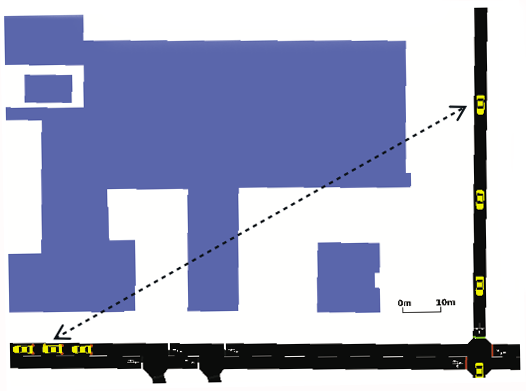
\includegraphics[width=.8\textwidth]{carpenter-1.png}
	\end{center}
	\label{fig:scenario-urbano-1}\caption{Esempio di scenario urbano.}
\end{figure}
%
Prendiamo l'esempio raffigurato in Figura~\ref{fig:scenario-urbano-1}, dove la linea fra i due veicoli interseca $n=6$ muri e una distanza interna di $d_o=32$m;
sostituendo i valori in~\ref{eq:osbtacle-model} si ottiene: $L_{s,o} = 9*6 + 0,4*32 = 66,8$dB.
Si evince come, con questa quantità di attenuazione, sia difficile che la trasmissione da un veicolo abbia abbastanza potenza per essere ricevuta dal secondo veicolo.
%
\section{L'implementazione}
%
\section{Utilizzo}
